\documentclass[tikz,border=7pt]{standalone}
\usepackage[T1]{fontenc}
\usepackage{lmodern}
\usepackage{amsmath}
\usepackage{tikz}
\usetikzlibrary{arrows.meta,calc,positioning}

\definecolor{itink}{RGB}{37,43,51}
\definecolor{itmuted}{RGB}{95,106,118}
\definecolor{itblue}{RGB}{54,128,191}
\definecolor{itgreen}{RGB}{57,145,112}
\definecolor{itorange}{RGB}{215,127,49}
\definecolor{itred}{RGB}{199,60,55}
\definecolor{itgray}{RGB}{245,247,250}

\begin{document}
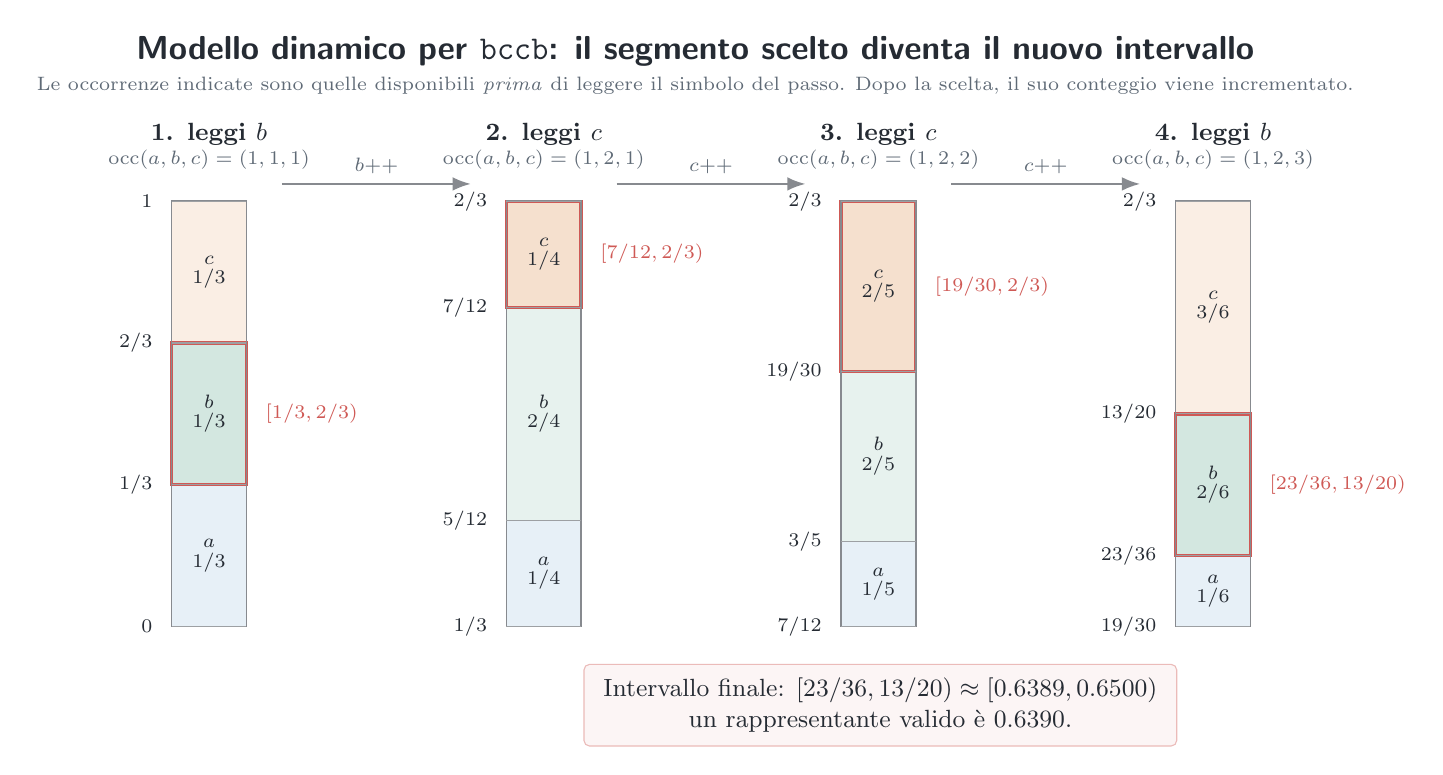
\begin{tikzpicture}[
    font=\sffamily,
    >=Latex,
    interval/.style={draw=itink!55, line width=0.55pt},
    boundary/.style={draw=itink!45, line width=0.45pt},
    arrow/.style={->, draw=itink!55, line width=0.8pt},
    selected/.style={draw=itred!85, line width=1.2pt},
    endpoint/.style={font=\scriptsize, text=itink, anchor=east},
    title/.style={font=\bfseries\small, align=center, text=itink},
    subtitle/.style={font=\scriptsize, align=center, text=itmuted},
    label/.style={font=\scriptsize\bfseries, align=center, text=itink}
]
    % Figure title and reading rule.
    \node[font=\sffamily\bfseries\large, text=itink] at (6.65,7.30)
        {Modello dinamico per \texttt{bccb}: il segmento scelto diventa il nuovo intervallo};
    \node[font=\scriptsize, text=itmuted, align=center] at (6.65,6.87)
        {Le occorrenze indicate sono quelle disponibili \emph{prima} di leggere il simbolo del passo. Dopo la scelta, il suo conteggio viene incrementato.};

    % Column x positions and common dimensions.
    \def\w{0.95}
    \def\xA{0}
    \def\xB{4.25}
    \def\xC{8.50}
    \def\xD{12.75}
    \def\h{5.4}

    % Step 1: current interval [0,1], probabilities (1/3,1/3,1/3), selected b.
    \node[title] at ($( \xA + 0.5*\w,6.25 )$) {1. leggi $b$};
    \node[subtitle] at ($( \xA + 0.5*\w,5.93 )$) {$\operatorname{occ}(a,b,c)=(1,1,1)$};
    \fill[itblue!12] (\xA,0) rectangle ++(\w,1.8);
    \fill[itgreen!22] (\xA,1.8) rectangle ++(\w,1.8);
    \fill[itorange!13] (\xA,3.6) rectangle ++(\w,1.8);
    \draw[selected] (\xA,1.8) rectangle ++(\w,1.8);
    \draw[interval] (\xA,0) rectangle ++(\w,\h);
    \foreach \y in {0,1.8,3.6,5.4} {
        \draw[boundary] (\xA,\y) -- ++(\w,0);
    }
    \node[label] at ($( \xA + 0.5*\w,0.9 )$) {$a$\\[-1pt]$1/3$};
    \node[label] at ($( \xA + 0.5*\w,2.7 )$) {$b$\\[-1pt]$1/3$};
    \node[label] at ($( \xA + 0.5*\w,4.5 )$) {$c$\\[-1pt]$1/3$};
    \node[endpoint] at ($( \xA - 0.12,0 )$) {$0$};
    \node[endpoint] at ($( \xA - 0.12,1.8 )$) {$1/3$};
    \node[endpoint] at ($( \xA - 0.12,3.6 )$) {$2/3$};
    \node[endpoint] at ($( \xA - 0.12,5.4 )$) {$1$};
    \node[font=\scriptsize, text=itred!85, anchor=west] at ($( \xA + \w + 0.12,2.7 )$) {$[1/3,2/3)$};

    % Step 2: current interval [1/3,2/3], probabilities (1/4,2/4,1/4), selected c.
    \node[title] at ($( \xB + 0.5*\w,6.25 )$) {2. leggi $c$};
    \node[subtitle] at ($( \xB + 0.5*\w,5.93 )$) {$\operatorname{occ}(a,b,c)=(1,2,1)$};
    \fill[itblue!12] (\xB,0) rectangle ++(\w,1.35);
    \fill[itgreen!12] (\xB,1.35) rectangle ++(\w,2.7);
    \fill[itorange!24] (\xB,4.05) rectangle ++(\w,1.35);
    \draw[selected] (\xB,4.05) rectangle ++(\w,1.35);
    \draw[interval] (\xB,0) rectangle ++(\w,\h);
    \foreach \y in {0,1.35,4.05,5.4} {
        \draw[boundary] (\xB,\y) -- ++(\w,0);
    }
    \node[label] at ($( \xB + 0.5*\w,0.675 )$) {$a$\\[-1pt]$1/4$};
    \node[label] at ($( \xB + 0.5*\w,2.7 )$) {$b$\\[-1pt]$2/4$};
    \node[label] at ($( \xB + 0.5*\w,4.725 )$) {$c$\\[-1pt]$1/4$};
    \node[endpoint] at ($( \xB - 0.12,0 )$) {$1/3$};
    \node[endpoint] at ($( \xB - 0.12,1.35 )$) {$5/12$};
    \node[endpoint] at ($( \xB - 0.12,4.05 )$) {$7/12$};
    \node[endpoint] at ($( \xB - 0.12,5.4 )$) {$2/3$};
    \node[font=\scriptsize, text=itred!85, anchor=west] at ($( \xB + \w + 0.12,4.73 )$) {$[7/12,2/3)$};

    % Step 3: current interval [7/12,2/3], probabilities (1/5,2/5,2/5), selected c.
    \node[title] at ($( \xC + 0.5*\w,6.25 )$) {3. leggi $c$};
    \node[subtitle] at ($( \xC + 0.5*\w,5.93 )$) {$\operatorname{occ}(a,b,c)=(1,2,2)$};
    \fill[itblue!12] (\xC,0) rectangle ++(\w,1.08);
    \fill[itgreen!12] (\xC,1.08) rectangle ++(\w,2.16);
    \fill[itorange!24] (\xC,3.24) rectangle ++(\w,2.16);
    \draw[selected] (\xC,3.24) rectangle ++(\w,2.16);
    \draw[interval] (\xC,0) rectangle ++(\w,\h);
    \foreach \y in {0,1.08,3.24,5.4} {
        \draw[boundary] (\xC,\y) -- ++(\w,0);
    }
    \node[label] at ($( \xC + 0.5*\w,0.54 )$) {$a$\\[-1pt]$1/5$};
    \node[label] at ($( \xC + 0.5*\w,2.16 )$) {$b$\\[-1pt]$2/5$};
    \node[label] at ($( \xC + 0.5*\w,4.32 )$) {$c$\\[-1pt]$2/5$};
    \node[endpoint] at ($( \xC - 0.12,0 )$) {$7/12$};
    \node[endpoint] at ($( \xC - 0.12,1.08 )$) {$3/5$};
    \node[endpoint] at ($( \xC - 0.12,3.24 )$) {$19/30$};
    \node[endpoint] at ($( \xC - 0.12,5.4 )$) {$2/3$};
    \node[font=\scriptsize, text=itred!85, anchor=west] at ($( \xC + \w + 0.12,4.32 )$) {$[19/30,2/3)$};

    % Step 4: current interval [19/30,2/3], probabilities (1/6,2/6,3/6), selected b.
    \node[title] at ($( \xD + 0.5*\w,6.25 )$) {4. leggi $b$};
    \node[subtitle] at ($( \xD + 0.5*\w,5.93 )$) {$\operatorname{occ}(a,b,c)=(1,2,3)$};
    \fill[itblue!12] (\xD,0) rectangle ++(\w,0.9);
    \fill[itgreen!22] (\xD,0.9) rectangle ++(\w,1.8);
    \fill[itorange!13] (\xD,2.7) rectangle ++(\w,2.7);
    \draw[selected] (\xD,0.9) rectangle ++(\w,1.8);
    \draw[interval] (\xD,0) rectangle ++(\w,\h);
    \foreach \y in {0,0.9,2.7,5.4} {
        \draw[boundary] (\xD,\y) -- ++(\w,0);
    }
    \node[label] at ($( \xD + 0.5*\w,0.45 )$) {$a$\\[-1pt]$1/6$};
    \node[label] at ($( \xD + 0.5*\w,1.8 )$) {$b$\\[-1pt]$2/6$};
    \node[label] at ($( \xD + 0.5*\w,4.05 )$) {$c$\\[-1pt]$3/6$};
    \node[endpoint] at ($( \xD - 0.12,0 )$) {$19/30$};
    \node[endpoint] at ($( \xD - 0.12,0.9 )$) {$23/36$};
    \node[endpoint] at ($( \xD - 0.12,2.7 )$) {$13/20$};
    \node[endpoint] at ($( \xD - 0.12,5.4 )$) {$2/3$};
    \node[font=\scriptsize, text=itred!85, anchor=west] at ($( \xD + \w + 0.12,1.8 )$) {$[23/36,13/20)$};

    % Update arrows between steps.
    \draw[arrow] ($( \xA + \w + 0.45,5.62 )$) -- node[above, font=\scriptsize, text=itmuted] {$b{+}{+}$} ($( \xB - 0.45,5.62 )$);
    \draw[arrow] ($( \xB + \w + 0.45,5.62 )$) -- node[above, font=\scriptsize, text=itmuted] {$c{+}{+}$} ($( \xC - 0.45,5.62 )$);
    \draw[arrow] ($( \xC + \w + 0.45,5.62 )$) -- node[above, font=\scriptsize, text=itmuted] {$c{+}{+}$} ($( \xD - 0.45,5.62 )$);

    % Final interval and transmitted representative.
    \node[
        draw=itred!35,
        fill=itred!5,
        rounded corners=2pt,
        inner xsep=7pt,
        inner ysep=5pt,
        align=center,
        font=\small,
        text=itink
    ] at (9.0,-1.0)
        {Intervallo finale: $\left[23/36,13/20\right)\approx[0.6389,0.6500)$\\
         un rappresentante valido \`e $0.6390$.};
\end{tikzpicture}
\end{document}
